\documentclass{sig-alternate}

\usepackage{listings}
\usepackage{url}
\usepackage{color}
\usepackage{multirow}
\usepackage[scaled=0.85]{helvet}
\usepackage{fullpage}

\newcommand{\Cpp}{C\kern-0.05em\texttt{+\kern-0.03em+}}
\newcommand{\conceptCpp}{Concept\Cpp}
\newcommand{\code}[1]{\lstinline[basicstyle=\sffamily]{#1}}
\newcommand{\func}[1]{\lstinline[basicstyle=\sffamily]{#1()}}
\newcommand{\ConceptCpp}{ConceptC\kern-0.05em\texttt{+\kern-0.03em+}}
\newcommand{\MPIpp}{MPI\kern-0.05em\texttt{+\kern-0.03em+}}
\newcommand{\Cilkpp}{Cilk\kern-0.05em\texttt{+\kern-0.03em+}}
\newcommand{\Charmpp}{Charm\kern-0.05em\texttt{+\kern-0.03em+}}
\newcommand{\tablefont}{\fontsize{8}{15}\selectfont}
\newcommand{\todoanju}[1]{\textcolor{blue}{Anju: #1}}
\newcommand{\todohaim}[1]{\textcolor{green}{Haim: #1}}
\newcommand{\todoamol}[1]{\textcolor{red}{Amol: #1}}
\newcommand{\todoanshul}[1]{\textcolor{cyan}{Anshul: #1}}
\newcommand{\halfline}{\vspace{-1.5ex}}

\lstdefinestyle{basic}{showstringspaces=false,
                       columns=fullflexible,
                       language=C++,
                       escapechar=@,
                       basicstyle=\normalsize\sffamily,
moredelim=**[is][\color{white}]{~}{~},
morekeywords={concept,model,require,where,reduction},
literate={->}{{$\rightarrow\;$}}1 {<-}{{$\leftarrow\;$}}1 {=>}{{$\Rightarrow\;$}}1,
}
 \lstset{language=C++,style=basic}

\begin{document}

%
% --- Author Metadata here ---
\conferenceinfo{SC}{'09 Portland, Oregon USA}

\title{PFunc: Modern Task Parallelism For Modern High Performance Computing}

\numberofauthors{5} 

\author{
% 1st. author
\alignauthor Prabhanjan Kambadur\\ \affaddr{Indiana University}\\
\email{pkambadu@osl.iu.edu}
% 2nd. author
\alignauthor Anshul Gupta\\ \affaddr{IBM T J Watson Research Center}\\
\email{anshul@us.ibm.com}
% 3rd. author
\alignauthor Amol Ghoting\\ \affaddr{IBM T J Watson Research Center}\\
\email{aghoting@us.ibm.com} \and  % use '\and' if you need 'another row' of
% 4th. author
\alignauthor Haim Avron\\ \affaddr{Tel-Aviv University}\\
\email{haima@post.tau.ac.il}
% 5th. author
\alignauthor Andrew Lumsdaine\\ \affaddr{Indiana University}\\
\email{lums@osl.iu.edu} }

\maketitle

\begin{abstract} 
HPC today faces new challenges due to paradigm shifts in both
hardware and software. The ubiquity of multi-cores, many-cores, and GPGPUs
is forcing traditional serial as well as distributed-memory parallel
applications to be parallelized for these architectures.  Emerging applications
in areas such as informatics are placing unique requirements on parallel
programming tools that have not yet been addressed.
%
Although, of all the available parallel programming models, task parallelism
appears to be the most promising in meeting these new challenges, current
solutions for task parallelism are inadequate.
%
In this paper, we introduce PFunc, a new library for task parallelism that
extends the feature set of current solutions for task parallelism with custom
task scheduling, task priorities, task affinities, multiple completion
notifications and task groups.
%
These features enable PFunc to naturally and efficiently parallelize a wide
variety of modern HPC applications and to support the SPMD model of parallel
programming.
%
We present three case studies: demand-driven DAG execution, frequent pattern
mining and iterative sparse solvers to demonstrate the utility of PFunc's new
features.  
\end{abstract}

\section{Introduction}
%2. Introduction - New architectures driving shared-memory and hybrid
%parallelism - Parallelization of applications in scientific computing is very
%well understood. But its mostly tied in to low level parallel constructs such
%as MPI -- this works on traditional clusters, but with finer grained
%parallelism becoming available, we need to switch to higher level APIs for
%parallel programming. These allow expression of parallelism sans the system
%details.  - Programmer productivity.  - New application domains such as
%informatics which were not kept in mind when designing the parallel interfaces
%we have today.  - How does PFunc address these issues. Specifically - New
%features - How are we evaluating them (Tell them what they can expect to take
%away from the paper) - Roadmap
Recent trends in hardware and software have brought new challenges to the HPC
community.  
% Hardware landscape has changed
The ubiquity of multi-core, many-core, and GPGPU architectures has had a
two-pronged impact. 
% 
First, it has necessitated parallelization of mainstream serial applications.
Parallelization of mainstream applications requires that the parallel
programming tools be palatable to common programmers.
% New applications are emerging
Also, large scale informatics applications have forced us to rethink the
parallel models that are traditionally employed to parallelize HPC
applications.  For example, most informatics applications have data sets that
are large, irregular and dynamic. These data sets and the corresponding
computations cannot be partitioned \textit{a priori}.  Therefore, these
applications are extremely sensitive to scheduling and load balancing, and
place unique requirements on the parallel programming tools. These
requirements have not yet been completely satisfied.  Second, traditional HPC
applications are being forced to parallelize for new cluster environments that
are made up of highly parallel, multi-core nodes.  These applications have been
developed for large distributed-memory computers using the single program
multiple data (SPMD)~\cite{darema2001} model, for which there is inadequate
support in existing shared-memory parallelization tools.

% Solution, task parallelism
Of the available parallel programming models, the task parallel model appears
to be the most promising in meeting these new challenges.  The task parallel
model is sufficiently high-level and generic, thereby enabling it to
parallelize regular and irregular applications on shared, distributed and
heterogeneous architectures alike.  However, current solutions for task
parallelism do not provide all the necessary features required for the
efficient parallelization of modern scientific computing, informatics, and
traditionally mainstream serial applications.  Execution parameters such as
task scheduling and task affinities are not exposed to the users. This
disallows user-driven customizations that are often critical to attaining good
application performance. Furthermore, lack of features such as task groups,
task priorities, and multiple task completion notifications prevents natural
expression of a wide variety of parallel algorithms including those normally
expressed in the SPMD model. Instead, users are forced to express their
algorithms in a manner that is less natural but more conducive to
parallelization by the parallel programming tool in use.

% Presenting PFunc
In this paper, we present PFunc, short for Parallel Functions, a lightweight
and portable library that provides C and C++ APIs to express task parallelism.
PFunc extends the features offered by current solutions for task parallelism
with customizable task scheduling, task priorities, task affinities, multiple
completion notifications and task groups. We demonstrate the utility of these
features by means of three case studies: (1) demand-driven execution of
directed acyclic graphs (DAGs), (2) frequent pattern mining, and (3) 
iterative sparse solvers. These case studies show that PFunc's new features enable
natural and efficient parallelization of a wide variety of modern HPC 
applications while also incorporating support for the SPMD parallel programming
model.
 
% Roadmap
The remainder of the paper is organized as follows.
Section~\ref{sec:background} gives a brief overview of existing models of task
parallelism and related work. 
% 
In Section~\ref{sec:shortcomings}, we briefly discuss the shortcomings of
current solutions for task parallelism.
%
In Section~\ref{sec:pfunc}, we introduce PFunc and describe its new features. 
%
In Section~\ref{sec:cases}, we study the effect of PFunc's new features on
parallelization of three different applications. 
%
Finally, in Section~\ref{sec:conclusion}, we draw conclusions from our studies
and briefly discuss future plans for PFunc.

\section{Background} \label{sec:background}
%3. Related work - Other efforts in parallel programming - HPCS - Cilk and
%others - Charm++, STAPL, etc.  Describe the Cilk model in some detail. We
%allude to this over and over.
The task parallel model breaks each program into individual tasks, and
subsequently, executes independent tasks in parallel.  Cilk~\cite{FrigoLeRa98},
an extension to the C language, is a popular solution for task parallelism.
The power of Cilk lies in its ability to dynamically schedule individual tasks
to achieve good parallel performance for many applications. At the heart of
Cilk is a provably efficient task scheduler that follows the
\textit{depth-first work, breadth-first steal} principle~\cite{Blumofe94}. Cilk
defines tasks as individual functions that may spawn other tasks.
Synchronization is effected by allowing tasks to wait on their children.
Cilk's execution model naturally imposes a tree structure on its programs.
Each thread executes its local subtree in a depth-first manner until it runs
out of work. When a thread exhausts all its work, it steals the shallowest
(closest to the root) task from a randomly chosen thread and continues
executing the stolen subtree. 

% Adherents of Cilk and others
Currently, there are many solutions for task parallelism that offer Cilk-style
semantics.  Of these, OpenMP 3.0~\cite{kn:omp_30}, Intel's Threading Building
Blocks (TBB)~\cite{kn:tbb}, Microsoft's Parallel Patterns Library (PPL), and
Task Parallel Library (TPL) are the most popular. 
% Java Concurrent Utilities 
Java Concurrent Utilities provides a work-sharing model of task parallelism.
% Other relevant solutions
Other relevant solutions that allow expression of task parallelism either
directly or indirectly include TPascal~\cite{Ansgar:1996},
STAPL~\cite{AnSTAPL01a, AnSTAPL01b}, HP\Cpp{}~\cite{gannon:hpc},
Fx~\cite{Gross:1994} and \Charmpp{}~\cite{Kale93charm++:a}.
% Compositional languages.
Task parallelism is also the design principle behind the compositional approach
to parallelism. This approach delivers parallelism by composing several
well-understood sequential components~\cite{Foster:1996p14161,
Abadi:1993p12637,Juan:1998p13476}. All compositions were implicitly parallel
and the possible interleavings of these components were controlled by
synchronization constructs. The compositional approach was embodied by both 
new languages (Strand~\cite{Foster:2008p806} and PCN~\cite{Foster:1996p14161}),
and by language extensions (C\Cpp~\cite{Chandy:1993p14898}, Fortran
M~\cite{Foster:1993p1441}).  This solution was elegant but was not broadly
applicable. 
%Parallel Skeletons
Another related approach to the compositional approach is called
\textit{parallel skeletons}~\cite{darlington93parallel,
boiten-transformational,
Cole:2004p14559,Kuchen:2002p14936,Bacci:1999p14920,Cole:1989p14916}. Parallel
skeletons have been used for the structured composition of parallel
programs~\cite{Darlington:1995p14933}. 
% HPCS
All of the three HPCS languages (Chapel~\cite{Chamberlain:2007p1040},
Fortress~\cite{fortress} and X10~\cite{Charles:2005p1232}) offer task
parallelism as language features. Of these, X10 differs from Cilk in that it
implements a \textit{breadth-first}~\cite{Cong08} work scheduling policy. Guo
et al.~\cite{Sarkar09} have recently proposed a hybrid model for work 
stealing. 
%
Bender and Rabin~\cite{BenderRa02} describe an online scheduler for
heterogeneous platforms that remedies the shortcomings of the Cilk scheduler 
for such platforms.
% Futures
Although semantically different from tasks, \textit{futures}~\cite{Halstead85}
offer features that are similar to the task parallel model in many respects.
Unlike tasks, futures are computations, which can be passed around and copied.
Notably, Cray XMT's Programming Environment~\cite{cray} provides first-class
futures.

% - Disadvantages of existing approaches - Show, don't tell - Provide specific
% examples - Use features that are missing that we will be using in the next
% section
%
% What is task parallelism and Cilk
\section{Shortcomings of current solutions for task parallelism}
\label{sec:shortcomings}
% Demand-driven DAG Scheduling
\begin{figure}[t] 
\centering 
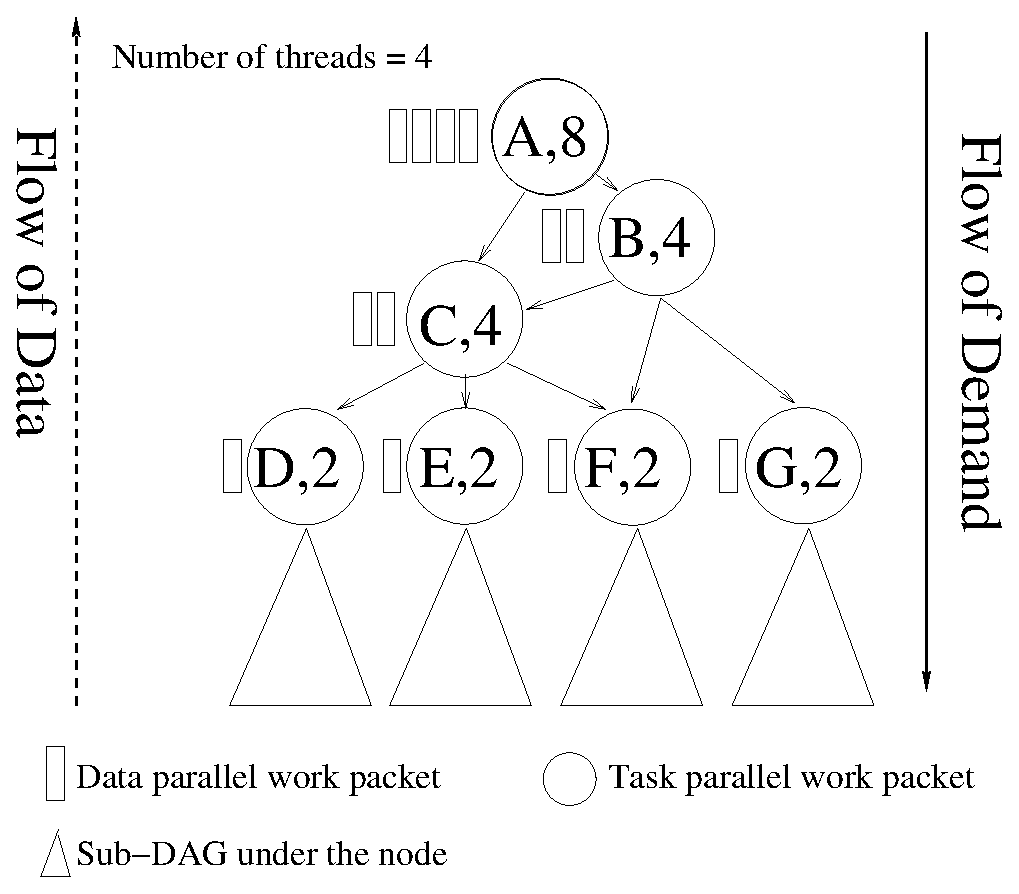
\includegraphics[width=0.08\textwidth]{figs/dag}
\caption{A simple DAG that cannot be directly parallelized using
the existing solutions for task parallelism.} 
\label{fig:dag} 
\end{figure}

In this section, we highlight some of the common shortcomings of the popular
solutions for task parallelism available today.  Current solutions for task
parallelism implement variations of the \textit{strict} computation
model~\cite{Blumofe94}, in which each task returns to exactly one ancestor.
Consequently, the overall task spawn structure in these solutions is a tree.
For example, consider the DAG in Figure~\ref{fig:dag} where the tasks A and B
must wait on task C to complete before they can continue their execution. This
simple DAG cannot be directly parallelized using any current task parallel
solution.  Support for multiple completion notifications is necessary to
exploit parallelism during the execution of such DAGs.  PFunc supports multiple
task completion notifications and enables parallelization of DAG executions
(see Section~\ref{sec:completions}).  Section~\ref{sec:dag} contains an
analysis of the performance implications of the lack of support for
parallelizing DAG executions in sparse factorizations.

% Frequent pattern mining
Currently, task scheduling is not exposed to the users. Furthermore, data
locality between tasks is exploited primarily through recursion.  For
non-trivial algorithms that are non-recursive, encoding data locality
implicitly by rewriting recursive versions 
of these algorithms is a challenging
prospect for the best of programmers.
%
Consider the sample execution of a level-wise frequent pattern mining algorithm
shown in Figure~\ref{fig:fim}. At each level, tasks that represent itemsets to
be mined are executed. Itemsets (and hence, tasks) to be mined at the next
level are generated \textit{only} after all the results from the previous
level are gathered (that is, there is no opportunity for recursion). In such
algorithms, there are significant opportunities to exploit data locality
between tasks at the same level (sibling tasks). For example, both tasks
(itemsets) AC and AE access A.  Existing scheduling policies do not take
advantage of such data locality.

% solution
As the data locality between tasks is highly application dependent, it is best
to provide users with the ability to customize task scheduling. 
%
In addition, users should be able to attach custom attributes such as
priorities to tasks that the scheduler can evaluate at runtime.  For example,
task priorities are essential to implementing a custom task scheduler for
real-time applications. PFunc offers users a wide variety of built-in scheduling
policies along with the ability to define their own custom scheduling policies. 
%
PFunc also provides task attributes, customizable task priorities, and
evaluation schemes for task priorities (see Section~\ref{sec:scheduling}).  The
performance implications of scheduling policies on informatics applications are
explored in detail in Section~\ref{sec:fim}.  Note that while PFunc
provides users the tools to customize task scheduling, it has
meaningful defaults that allow them to be completely
oblivious to the scheduling details.

\begin{figure}[t]
\centering
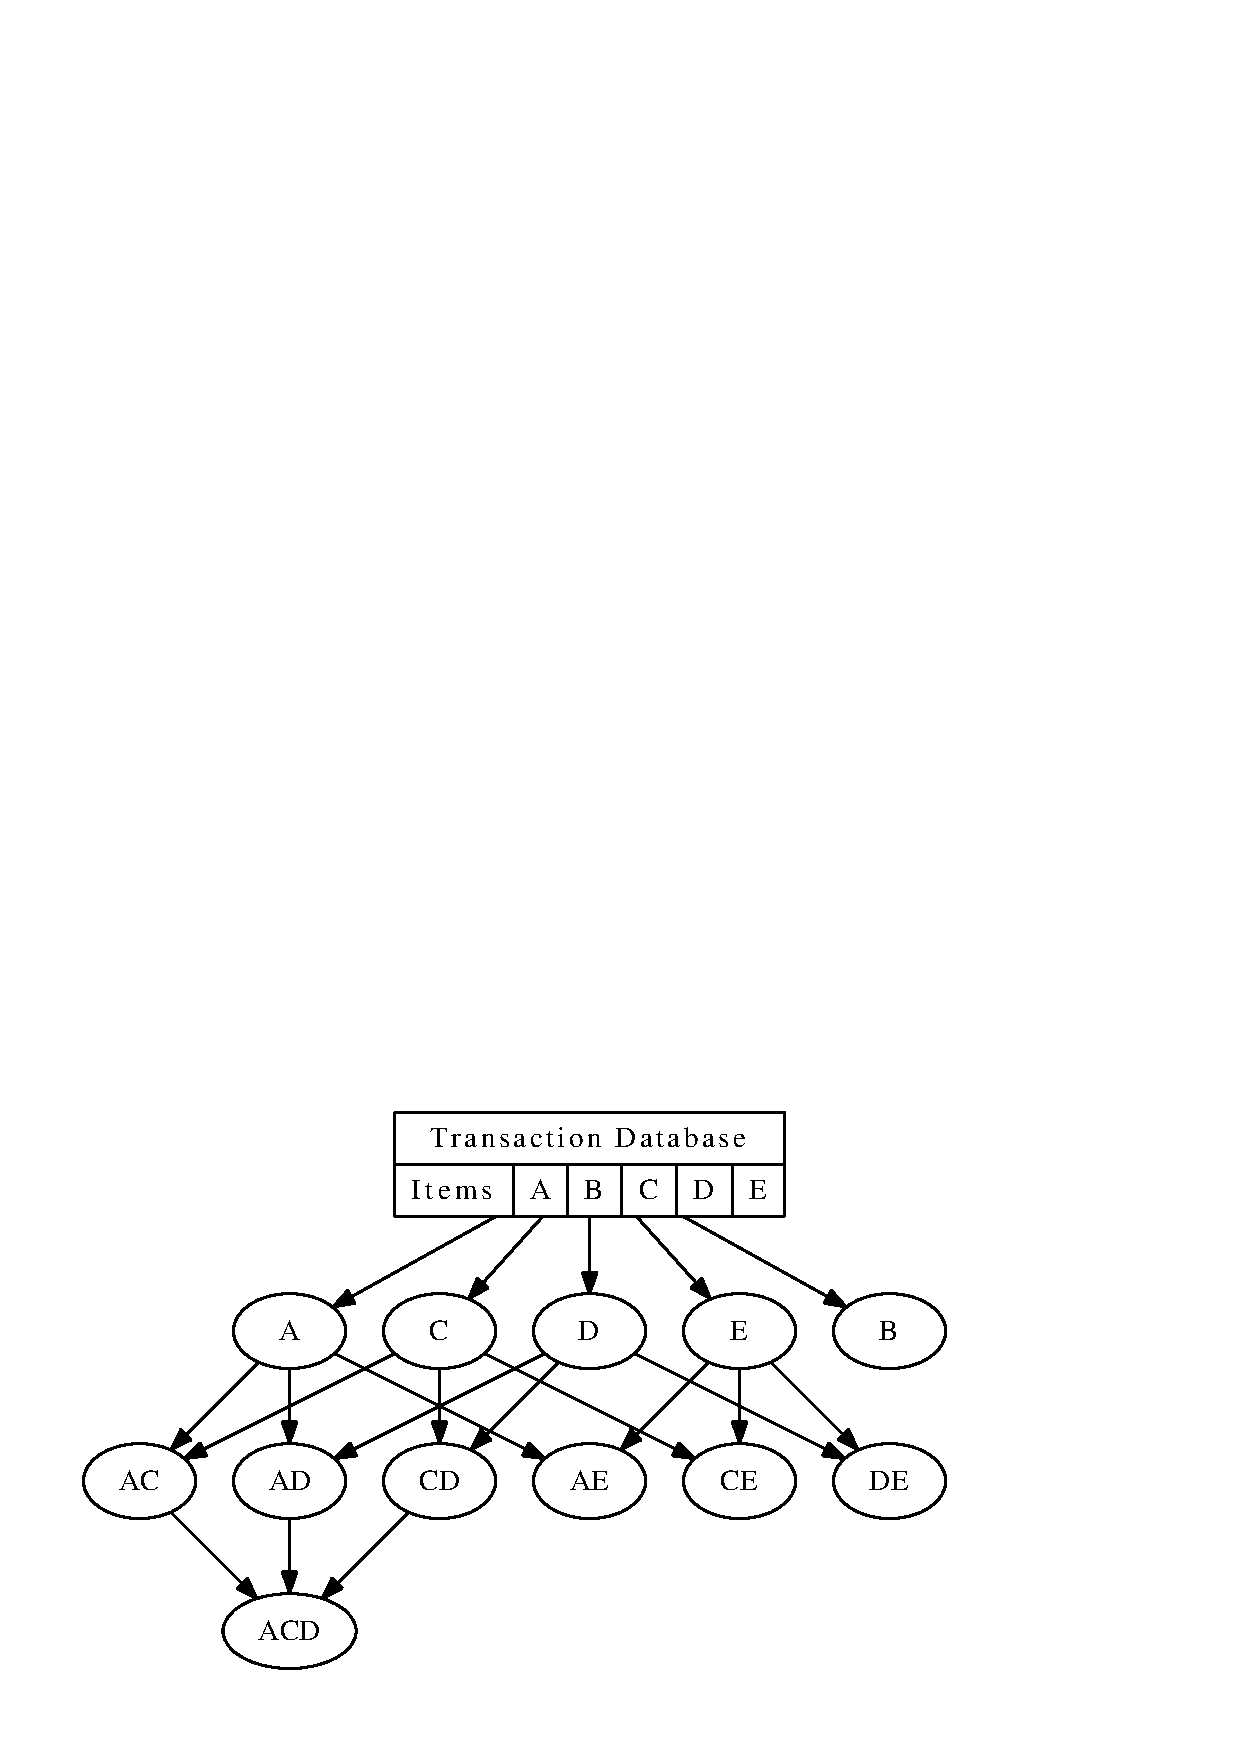
\includegraphics[width=0.30\textwidth]{figs/itemset}
\caption{A frequent pattern mining algorithm that can not be efficiently
parallelized by the existing task parallel implementations.}
\label{fig:fim}
\end{figure}
 
% Iterative sparse solver
Many parallel algorithms are best expressed in the SPMD model where groups of
cooperating tasks alternate between communication and computation to solve a
particular problem.  Iterative solvers such as conjugate gradient (CG) and
GMRES~\cite{saadBook}, and graph algorithms such as shortest
paths~\cite{Meyer03:DeltaStepping} are best parallelized using this model.
However, current solutions for task parallelism do not incorporate support for
the SPMD model and therefore, force users to rewrite of the original SPMD-parallel
algorithms.  This not only results in wasted effort, but might also degrade
application performance by destroying the natural locality that is typical of
SPMD programs.  PFunc supports the natural expression of SPMD algorithms
through its task group mechanism (see Section~\ref{sec:groups}).  In
Section~\ref{sec:cg}, we study the performance implications of the lack of
support for the SPMD model in current solutions as applied
to iterative sparse solvers.

% Task affinities
To maintain scalability and continued performance increments in the face of the
microprocessor clock frequency ceiling, modern computing platforms are rapidly
embracing heterogeneity and Non-Uniform Memory Access (NUMA).  For example, AMD
Opteron is NUMA-based, and Intel's Larrabee~\cite{seiler2008} is both
heterogeneous and NUMA-based. These architectures impose an additional
constraint of affinity on both tasks and threads to obtain good performance.
Current solutions for task parallelism do not allow users to set affinities of
tasks to queues and ultimately, to processors. 
%
Without this feature, task parallelism will be unable to serve as the parallel
platform for modern HPC. PFunc allows users to fully
exploit heterogeneous environments through its support for task
affinities (see Section~\ref{sec:affinities}).

\section{PFunc}
\label{sec:pfunc}
%  - Give people a flavor of whats going on.
%    - Task parallel library
%    - Hello world -- fibonacci
%  - What is significantly different. describe only those features
%    that are different.
%    - One or two inlined calls that depict how to utilize the feature.
%  - Describe all the features for completeness.
%    - This is important to point out that we are a superset of TBB and Cilk
%      and OpenMP.

\begin{figure*}[t]
\centering
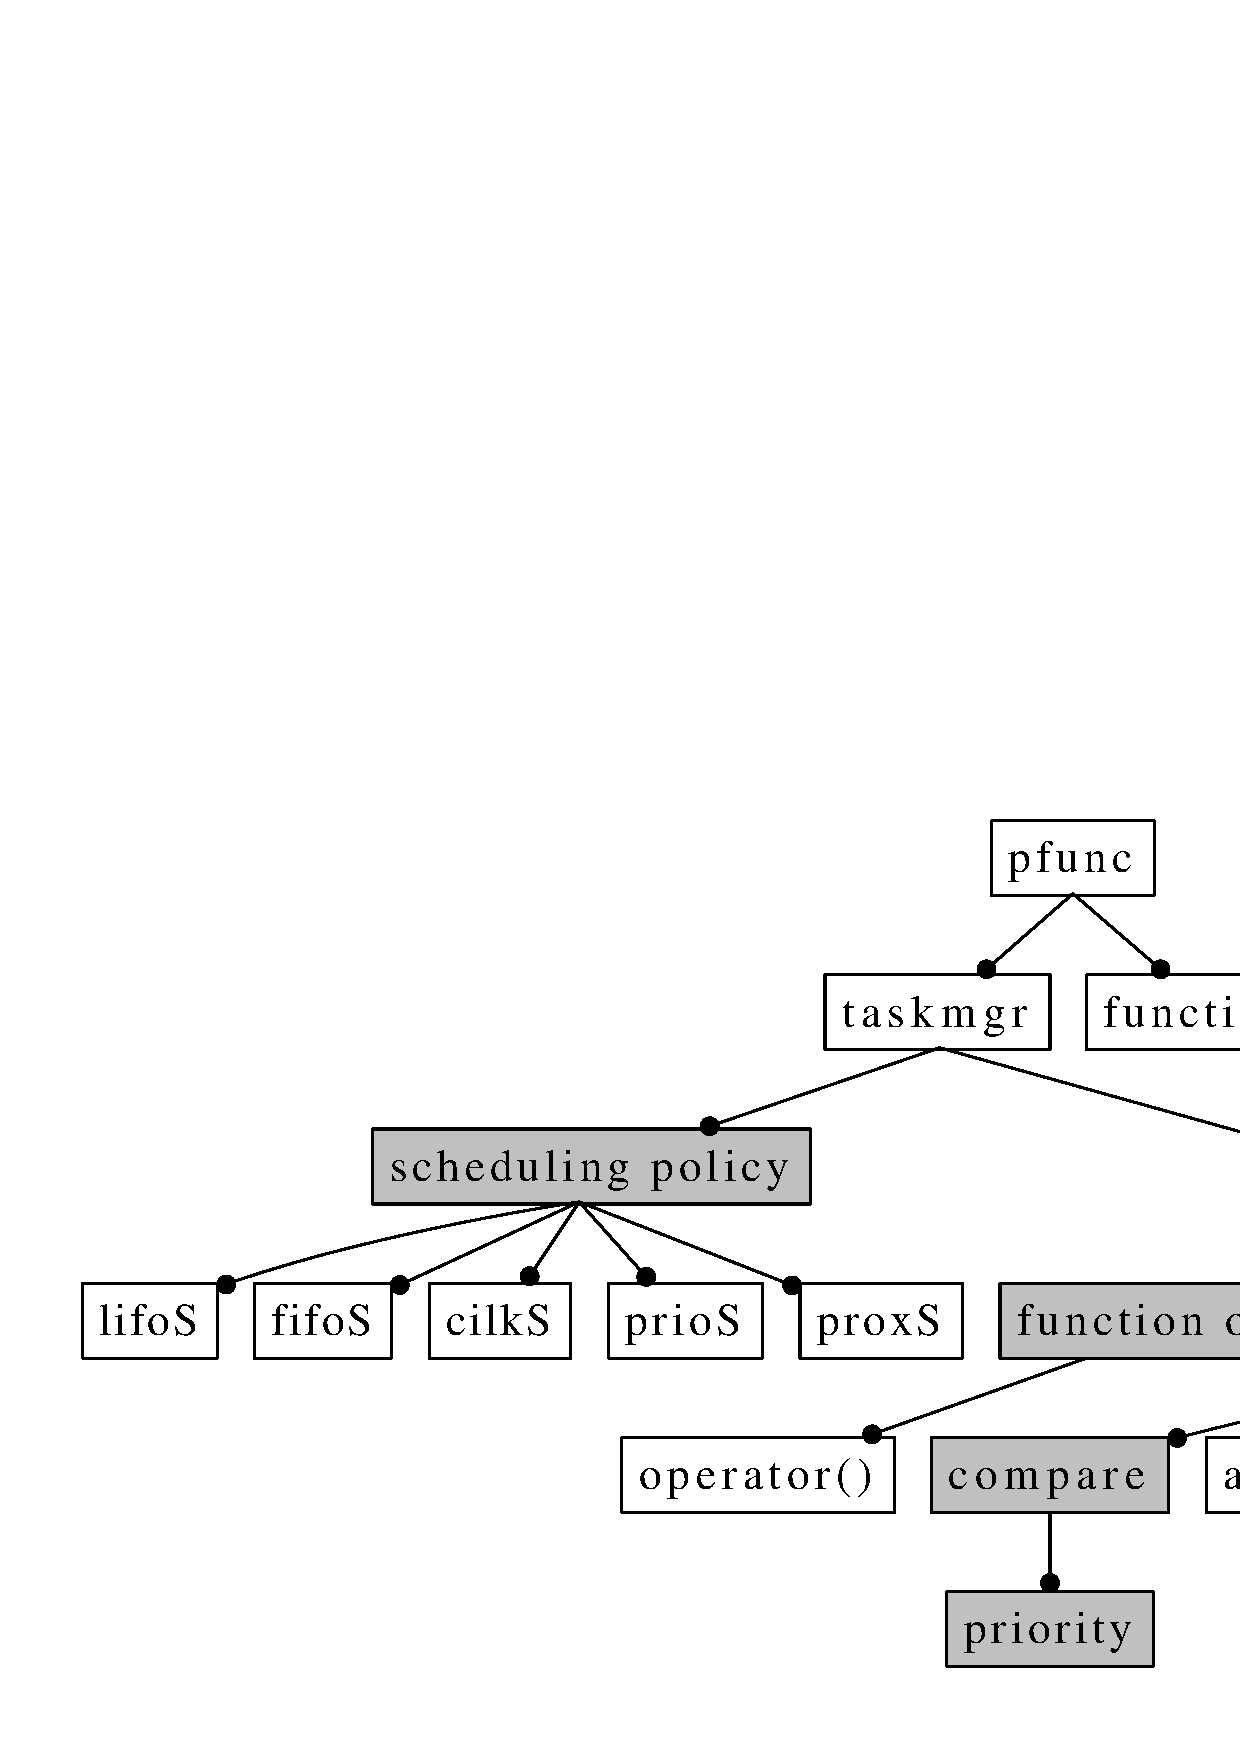
\includegraphics[width=0.90\textwidth]{figs/pfunc}
\caption{Feature diagram of the PFunc library showing the various features.
The features colored grey (scheduling policy, function object, compare and
priority) are generated based on user input.}
\label{fig:pfunc}
\end{figure*}

PFunc, short for Parallel Functions, is a lightweight and portable library that
provides C and \Cpp{} APIs to express task parallelism. The features offered by
PFunc are a strict superset of the features offered by current solutions for
task parallelism.  Specifically, PFunc extends the feature set of current
solutions with custom task scheduling, task priorities and task affinities.
Furthermore, PFunc offers task groups for SPMD-style programming and multiple
task completion notifications for parallel execution of DAGs.  PFunc's extended
feature set is geared towards helping knowledgeable users optimize their
application performance. In this section, we describe PFunc with an emphasis on
its new features.  Due to space constraints, all the code samples given in this
section are in \Cpp{}. All the functionality described in this section is also
available through PFunc's C interface.

% Explain the architecture
\subsection{Design overview}
\label{sec:design}
PFunc's design is based on the principles of generic and generative
programming. As a result, PFunc is able to offer a wide variety of
customizations to its users without incurring any runtime penalties.  Using
PFunc is a two step process. First, users generate a customized library
instance description that best suits their needs using PFunc's \code{generator}
interface. Second, the generated library instance description is used to
parallelize user applications. A feature diagram of PFunc is shown in
Figure~\ref{fig:pfunc}. The shaded blocks represent features that
can be customized and are described below.
\begin{list}{\labelitemi}{\leftmargin=1em}
% Scheduling policy
\item \textbf{Scheduling policy:}
The value provided to this feature determines the scheduling policy that is
used in the generated library instance description.  Figure~\ref{fig:pfunc}
enumerates all the built-in values that can be provided for this feature.
PFunc's users can also define custom scheduling polices and use them as the
value of this feature at instance generation time.
% Compare
\item \textbf{Compare:}
This feature represents the ordering function for task priorities and is used
only if the chosen scheduling policy requires task priorities. PFunc also
allows customization of the \textbf{priority} feature as it is inherited from
the \textbf{compare} feature.
% Functor
\item \textbf{Function object:}
This feature allows users to specify the type of the function object that is
executed by the tasks.  By allowing the type of the function object to be
specified as a feature, PFunc successfully avoids paying the cost of virtual
function calls in the spawned tasks. This is unlike other library-based
approaches such as TBB where spawning a new task involves a virtual function
call.  
\end{list}

For example, consider the following piece of code:

\begin{lstlisting}
typedef pfunc::generator<cilkS, /* scheduling policy */
                          use_default, /* compare */
                          use_default> my_pfunc; /*function object*/
\end{lstlisting}

Here, we have generated an new library instance description of PFunc by
choosing the Cilk-style scheduling policy. The values for the \textbf{compare}
and \textbf{function object} features are allowed to be defaults.~\footnote{It
is possible to use \code{use_default} for all the features.
PFunc automatically chooses sensible defaults in this case.}
The type \code{my\_pfunc} thus generated is a custom instance that can be used
to parallelize user applications. In PFunc, there are four important types that
users are exposed to.  These are: \code{attribute},
\code{group}, \code{task} and \code{taskmgr}.  Once the required library
instance description has been generated, these types can be accessed as
follows:

\begin{lstlisting}
my_pfunc::attribute attr; 
my_pfunc::group grp; 
my_pfunc::task tsk; 
my_pfunc::taskmgr tskmgr; 
\end{lstlisting}

% attribute
Objects of type \code{attribute} allow users to control the execution of
spawned tasks by setting attributes such as task priority and task affinity. 
% group
Objects of type \code{group} can be used to create collaborations of tasks that
can communicate with each other using point-to-point message passing and
barrier synchronization.
% task
Objects of type \code{task} are used as references to spawned tasks, which 
can be passed to other tasks. The ability to pass task references is crucial
for the support of multiple task completion notifications.
% taskmgr
Finally, objects of type \code{taskmgr} manage threads and their task
queues, and are responsible for task scheduling. 

% Fibonacci
Figure~\ref{fig:hello_world} demonstrates how computation of Fibonacci numbers
can be parallelized using PFunc. When the Fibonacci number that needs to be
calculated is a non-base case ($N\ge2$), two new tasks are spawned (using
\func{spawn}) to calculate the $(N-1)^{st}$ and $(N-2)^{nd}$ Fibonacci numbers.
Each task waits (using \func{wait}) for both of its sub-tasks to complete
before adding the results up. 
%
To generate the library instance description of PFunc for the execution of our
Fibonacci example, we choose Cilk-style scheduling.  As task priorities are not needed,
we use \code{use\_default} for the \textbf{compare} feature.  Finally, we
specify the type \code{fibonacci} as the value of the \textbf{function object}
feature.

% A simple example
\begin{figure}[t]
\begin{center}
\begin{lstlisting}[frame=lrtb]
struct fibonacci; /*forward declaration*/
typedef pfunc::generator <cilkS, use_default, fibonacci> my_pfunc;
my_pfunc::taskmgr fib_taskmgr; /*assume to be initialized*/
@\halfline@
struct fibonacci {
  const int n; int fib_n;
@\halfline@
  fibonacci (const int& n) : n(n), fib_n(0) {}
@\halfline@
  void operator () (void) {
    if (0 == n || 1 == n) fib_n = n;
    else { 
      my_pfunc::attribute fib_attr;
      my_pfunc::group fib_group;
      my_pfunc::task tsk_n_1, tsk_n_2;
      fibonacci fib_n_1 (n-1);
      fibonacci fib_n_2 (n-2);
@\halfline@
      pfunc::spawn (fib_taskmgr, tsk_n_1, fib_attr, fib_group, fib_n_1);
      pfunc::spawn (fib_taskmgr, tsk_n_2, fib_attr, fib_group, fib_n_2);
@\halfline@
      pfunc::wait (fib_taskmgr, tsk_n_1);
      pfunc::wait (fib_taskmgr, tsk_n_2);
@\halfline@
      fib_n = fib_n_1.fib_n + fib_n_2.fib_n;
    }
  } 
};
\end{lstlisting}
%\vspace{-5pt}
\caption{Parallel Fibonacci numbers using PFunc.}
%\vspace{-10pt}
\label{fig:hello_world}
\end{center}
\end{figure}


\subsection{Initializing PFunc}
\label{sec:initializing}
Once the appropriate types have been generated, users are required to
initialize at least one object of type \code{taskmgr} that will
schedule and run the spawned tasks. For example, we can initialize the
\code{fib\_taskmgr} object in the Fibonacci example in
Figure~\ref{fig:hello_world} in following manner:

\begin{lstlisting}
const unsigned int num_queues = 4; 
const unsigned int threads_per_queue[] = {1, 1, 1, 1}; 
taskmgr fib_taskmgr (num_queues, threads_per_queue);
\end{lstlisting}

This creates \code{fib\_taskmgr}, an object of type \code{taskmgr}, with four
task queues and one thread per task queue. PFunc allows a $m\times{}n$ with
$(m\le{}n)$ mapping between the task queues and threads. A $m==n$ mapping is
similar to Cilk where each thread has its very own task queue. Threads'
processor affinities can be set using an optional third argument to the
constructor of \code{taskmgr} (see Section~\ref{sec:affinities}).

\subsection{Scheduling policy and task priority}
\label{sec:scheduling}
PFunc allows users to choose the scheduling policy through its \code{generator}
interface. For the Fibonacci example shown in Figure~\ref{fig:hello_world}, we
used the Cilk-style scheduling policy (\code{cilkS}). In addition to
\code{cilkS}, PFunc provides first-in first-out (\code{fifoS}), last-in
first-out (\code{lifoS}), priority-based (\code{prioS}) and proximity-based
(\code{proxS}) scheduling policies.  Consider the following example that
chooses the priority-based scheduling policy:

\begin{lstlisting}
typedef pfunc::generator<prioS, std::less<int>, use_default> gen; 
typedef gen::taskmgr taskmgr;
typedef gen::attribute attribute;
@\halfline@
taskmgr my_taskmgr (...);
attribute my_attr;
pfunc::attr_priority_set (my_attr, 10);
pfunc::spawn (my_taskmgr, /*task*/, my_attr, /*group*/, /*fn object*/);
\end{lstlisting}

Apart from choosing priority-based scheduling, we have also chosen to use
\code{int}s (implicitly) as task priorities and \code{std::less<int>} to
compare task priorities. Now, each task is attached to an integer priority
that determines its execution schedule. Task priorities are accessed  using
objects of type \code{attribute}. In the code example above, we spawn a task
using $10$ as its priority. Note that we can use \textit{any} suitable type as
the task priority and the ordering function. The proximity-based scheduling
policy utilizes k-d trees~\cite{bentley:1975} to dynamically choose the next
task to be executed.  This scheduling policy is employed in situations where
the task priorities are best represented as spatial coordinates in
n-dimensional Euclidean space. In addition to these built-in scheduling
policies, user-defined scheduling policies can also be used. 

Much like \code{cilkS}, work-stealing is employed in the \code{fifoS},
\code{lifoS}, \code{prioS} and \code{proxS} scheduling policies to load balance
applications runs. However, the choice of the victim task  depends  on the
scheduling policy in use. For example, in \code{prioS}, the stolen task is
always the highest priority task in the victim thread's queue. This ensures
that a task's priority is respected even in the case of a steal.

\subsection{Completion notifications}
\label{sec:completions}
With respect to task completion notifications, PFunc departs from current
solutions for task parallelism in two ways. First, PFunc does not follow the
strict computation model~\cite{Blumofe94}. Therefore, a task's completion
notification can be delivered to a non-ancestor task. Second, PFunc supports
multiple task completion notifications, and therefore, multiple tasks are
allowed to wait on the completion of the same task. Hence, PFunc inherently
supports parallel execution of DAGs.  The example below shows how multiple task
completion notifications can be enabled for a task. 

\begin{lstlisting}
task my_task;
attribute my_attr;
pfunc::attr_num_waiters_set (my_attr,4/*four parents*/);
pfunc::spawn (/*taskmgr*/, my_task, my_attr, /*group*/, /*fn object*/);
...
pfunc::wait (/*taskmgr*/, my_task);
\end{lstlisting}

In this example, we first set the number of completion notifications to be
delivered for a particular task to $4$ using the attribute associated
with the task. Once the call to \func{spawn} returns, \code{my_task} can be
used to wait on the completion of the spawned task. In order to enable other
tasks to wait on the currently spawned task, references to \code{my_task} must
be passed to those tasks by the spawning task.

\subsection{Task groups}
\label{sec:groups}
As it is difficult to express all segments of a program in the task parallel
model, PFunc allows users to mix task parallelism with SPMD-style programming
through the use of task groups.  Tasks within the same group can communicate
using built-in point-to-point and collective operations.  The following example
demonstrates the use of groups:

\begin{lstlisting}
attribute my_attr;
group my_group;
pfunc::attr_grouped_set (my_attr, true /*use groups*/);
pfunc::group_id_set (my_group, 1234 /*for debugging*/);
pfunc::group_size_set (my_group, 2 /*num tasks in group*/);
pfunc::spawn(my_taskmgr, /*task1*/, my_attr, my_group, /*fn object*/);
pfunc::spawn(my_taskmgr, /*task2*/, my_attr, my_group, /*fn object*/);
\end{lstlisting}

First, we enable grouping by turning on the \code{grouped} attribute for the
tasks. Next, we set up \code{my\_group} to have an id of $1234$ and contain $2$
members. When the tasks are spawned, each of them is assigned a rank in the
group that can be used for communication purposes. Groups provide tasks that
need frequent synchronization a clean interface through collective operations
such as barriers.  PFunc provides three kinds of barriers: spinning, waiting
and stealing. The example below demonstrates how the kind of barrier executed
can be changed.

\begin{lstlisting}
group my_group;
pfunc::group_barrier_set (my_group, BARRIER_SPIN);
\end{lstlisting}

The spinning barrier (default) can be used when the wait time is expected to be
small. On the other hand, the waiting barrier can be used when the wait times
are expected to be large. In a stealing barrier, a thread that is executing a
task that is waiting on a barrier, is free to select and execute tasks from
other groups. 

\subsection{Task affinities}
\label{sec:affinities}
PFunc allows users to control the affinity of their tasks to task queues, and
in turn, to threads and CPUs.  This enables PFunc's users to fully utilize
modern computer architectures, which are inherently heterogeneous.  By
default, PFunc enqueues newly spawned tasks onto the queue of the spawning
thread. However, users can override this default and place individual tasks
onto particular queues.  

\begin{lstlisting}
const unsigned int nqueues = 2;
const unsigned int nthds_per_queue = {2,2};
const unsigned int thd_affinities [2][2] = {{0,1},{2,3}};
@\halfline@
taskmgr my_taskmgr (nqueues, nthds_per_queue, thd_affinities);
attribute my_attr;
pfunc::attr_affinity_set (my_attr, 1);
pfunc::spawn (my_taskmgr, /*task*/, my_attr, /*group*/, /*fn object*/);
\end{lstlisting}

In the above example, two task queues having two threads each are created. The
four threads are bound to CPUs $0, 1, 2$ and $3$, respectively, using the
optional third argument to \code{my\_taskmgr}. Finally, the task's affinity is
set to task queue $1$ using \code{my\_attr}. Therefore, the task is spawned
on the first queue where it is executed either by thread 0 or thread 1 (that
is, on CPU 0 or 1).

\subsection{Exception handling}
\label{sec:exceptions}
PFunc provides an elegant exception handling mechanism that delivers exceptions
thrown by a task across threads to the task that is waiting on it. In the case
that the task throwing the error has more than one task waiting on it, the
thrown error object is delivered to each of the waiting tasks. The code sample
below demonstrates the use of PFunc's exception handling mechanism.

\begin{lstlisting}
struct my_fn_object { 
  void operator () { 
    try { ... }
    catch (const pfunc::exception& error) { 
      std::cout << error.what () << error.trace () << error.code (); 
    } 
  }
};
\end{lstlisting}

PFunc's exceptions extend \code{std::exception} with two new functions. The
member \func{exception::trace} returns the stack trace of the calls through
which this exception object was transported. The function
\func{exception::code} is useful when the exception was caused by a system call
and returns the error number.  For performance, exception handling is
disabled by default and can be enabled using a compile time flag. 

\subsection{Performance profiling}
\label{sec:performance}
PFunc is fully integrated with the Performance Application Programming
Interface (PAPI)~\cite{papi}, thereby allowing users to profile their
applications with ease. PAPI was chosen due to its wide availability and
portability across many hardware platforms. Profiling is handled mainly through
the \code{taskmgr} type. Users can specify the events (both PAPI presents and
native) that they wish to monitor when initializing objects of the
\code{taskmgr} type. Consider the sample code given in Figure~\ref{fig:perf}.
In this example, we utilize PFunc to measure L1 data cache behavior. We
derive from \code{perf\_data} to communicate the required
measurements to PFunc. PFunc stores the requested event values in
\code{my\_perf\_data} and these values can subsequently be used for performance
tuning.

\begin{figure}[t]
\centering
\begin{lstlisting}[frame=trbl]
enum {nthds=2,nevents=2};
@\halfline@
struct my_perf_data: pfunc::perf_data {
  perf_data::event_value_type storage[nthds][nevents];
  int events[nevents];
@\halfline@
  my_perf_data () {
    events[0] = PAPI_L1_DCA; 
    events[1]= PAPI_L1_DCM;}
  }
@\halfline@
  int get_num_events () const { return nevents; }
@\halfline@
  int* get_events () const { return events; }
@\halfline@
  perf_data::event_value_type** get_event_storage () const {
    return storage; 
  }
}
@\halfline@
my_perf_data perf;
taskmgr my_taskmgr (/*nqueues*/, /*nthreads_per_queue*/, perf);
\end{lstlisting}
\caption{A code segment that uses PFunc's integration with PAPI to measure its
L1 cache behavior.}
\label{fig:perf}
\end{figure}

\section{Case Studies}
\label{sec:cases}
In Section~\ref{sec:pfunc}, we explored the new features introduced by PFunc in
addition to the features offered by current solutions for task parallelism. In
this section, we study the utility of some of these new features through three
case studies.

\subsection{Demand-driven DAG execution}
\label{sec:dag}
%   - DAG scheduling
%    - Background and what is the unique requirement placed by this 
%      application.
%    - Description of how this can be done in the existing model. 
%    - Description of how this can be done using PFunc's new features.
%    - Results
Program execution is often modeled as the execution of a DAG $G=(V,E)$ where
the vertex set $V$ represents computations and the edge set $E$ represents data
dependencies (communications). Such \emph{dataflow} schemes are an excellent
means of expressing  application-level parallelism.  The dataflow model can be
classified based on the order in which the computations (vertices) encoded by
the DAG are executed. In the \textit{demand-driven} dataflow model,
computations are initiated when there is a demand for data.  Conversely, in the
\textit{data-driven} dataflow model, computations are initiated as and when
those computations' inputs become available.  Both the demand-driven and the
data-driven models are important programming paradigms of the dataflow model,
and are applicable in different scenarios. 

The demand-driven model for the execution of dataflow DAGs offers many benefits
over the data-driven model. First, as the data is only produced on demand, the
lifetime of the produced data, and consequently the application's memory
footprint, can be effectively reduced. Second, the demand-driven model
facilitates recursive partitioning of the compute resources and therefore,
lends itself to elegant scheduling.  However, current solutions for task
parallelism do not support parallelization of the demand-driven execution of
DAGs. In this case study, we describe the requirements placed by the
demand-driven model on task parallelism.  Furthermore, we parallelize the
execution of a sparse unsymmetric LU factorization algorithm using both the
data-driven and demand-driven models to characterize the effects of the
parallel execution model on application performance. For a more detailed 
discussion of the current case study, please refer to Kambadur et
al.~\cite{kambadur09:dag}.

\paragraph{Problem description}
The sparse unsymmetric-pattern multifrontal algorithm for LU factorization with
partial pivoting used in our study was described by
Gupta~\cite{GUPTAsimax01,GUPTA00wsmp2}. This algorithm uses a DAG
representation and the demand-driven dataflow model for an efficient
parallel implementation on multi-core processors.  During the symbolic phase of
this algorithm, it generates a task DAG, $G =(E,V)$, where each vertex $v \in
V$ represents a frontal matrix and each edge $(u \rightarrow{} v) \in E$
represents a data dependency from vertex $u$ to $v$.  When a vertex  (task) in the task DAG is
executed, it performs a supernodal dense LU factorization step and the
resulting update matrix is used by dependent vertices for their computations.
The memory required for the update matrix is allocated by the computing vertex,
and can only be deallocated when all of the data in the update matrix has been
processed by the dependent vertices.  Therefore, for ideal performance, it is
essential to schedule the tasks such that the memory allocated by a task can be
freed as soon as possible. The task DAG produced by the symbolic phase can be
executed in both the data-driven and the demand-driven models. However, by
virtue of spawning new tasks only when the data is required, the demand-driven
model promises to be more memory efficient than the data-driven model.

\paragraph{Requirements placed on task parallelism}
In the demand-driven model, when a task completes, \textit{all} its parents
should be notified so that they can consume the resulting data.  This requires
that the tasking solution support multiple notifications. 

\paragraph{Shortcomings of current solutions}
Current solutions for task parallelism implement different variations of the
strict computation model. Consequently, multiple task completion
notifications are not supported.  Support for multiple notifications is a hard
requirement that is essential for the correctness and the efficiency of the
demand-driven model.  One can remedy the lack of multiple notification support
by resorting to using system-level synchronization constructs such as locks and
condition variables to provide application-level notifications.  However, such
remedies have two drawbacks. First, as locks and condition variables operate at
the scope of threads and not tasks, they block the entire thread instead of
just a single task. Second, resorting to low-level constructs such as locks and
condition variables can result in unsafe and unmaintainable code.  When
multiple task completion notifications are supported by the tasking library
itself, a thread that is executing a task that is waiting on other tasks to
complete, is free to select and execute another task from the list of runnable
tasks.

\paragraph{PFunc's approach}
Parallelizing the demand-driven execution of DAGs using PFunc is
straight-forward as PFunc supports multiple task completion notifications(see
Section~\ref{sec:completions}). 

\paragraph{Experimental results}
\begin{figure}[t]
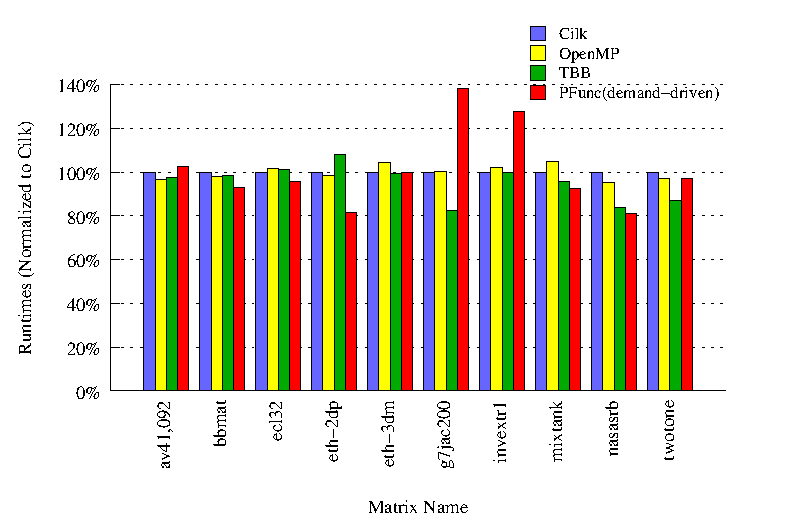
\includegraphics[width=0.5\textwidth]{dagresults/dag_speedup}
\caption{Performance of various DAG execution implementations relative to Cilk
when using 8 threads.}
\label{fig:dag_speedup}
\end{figure}

\begin{figure}[t]
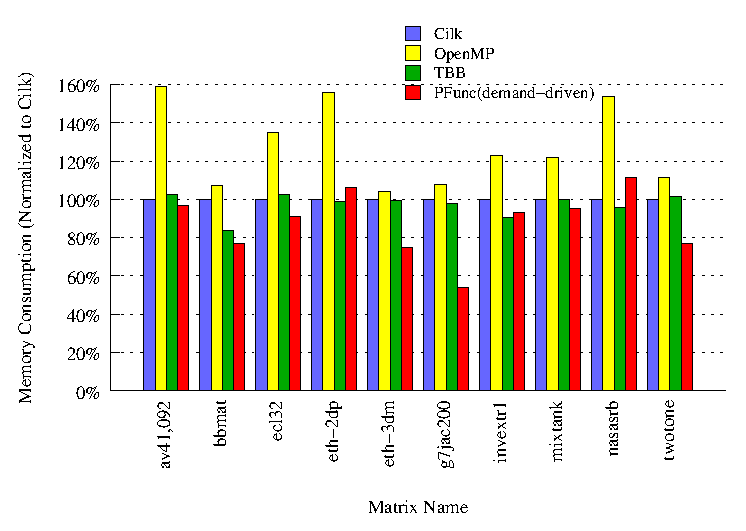
\includegraphics[width=0.5\textwidth]{dagresults/dag_memory}
\caption{Peak memory consumption of various DAG execution implementations 
relative to Cilk when using 8 threads.}
\label{fig:dag_memory}
\end{figure}

To benchmark the performance of the sparse unsymmetric multifrontal algorithm
for LU factorization using the demand-driven model, we implemented the
data-driven model using Cilk, OpenMP and TBB. PFunc was used to parallelize
the demand-driven model.  For the Cilk implementation, we used the Cilk 5.4.6
compiler.  The TBB implementation used the GCC 4.3.2 compiler with TBB 2.1.
PFunc implementations were also compiled with GCC 4.3.2. Because of its
excellent support for tasks, we used Sun CC 5.10 for the OpenMP
implementation. 
%
The tests were run on a dual Intel Xeon x5365 processor using Linux 2.6.27. The
benchmarks were run on matrices from the University of Florida Sparse Matrix
Collection~\cite{davissparse}.

% Explain the results
Figure~\ref{fig:dag_memory} shows the peak memory consumption of the data- and
demand-driven implementations with 8 threads relative to Cilk.  We see that the
memory consumption for the demand-driven execution is lower than that of the
data-driven implementations on average.  Figure~\ref{fig:dag_speedup} shows the
application runtimes of the data- and demand-driven implementations with 8
threads relative to Cilk.  We see that demand-driven execution performs
comparably to other data-driven execution schemes. Some variance exists among
the data-driven model implementations due to the differences in the
implementations of the task parallel solutions themselves. 
% Conclude
When taken in tandem, Figures~\ref{fig:dag_speedup} and~\ref{fig:dag_memory}
allows us to conclude that the demand-driven model shows promise to decrease
the memory requirements of many sparse matrix computations without losing
performance in comparison to the data-driven execution model. 

\subsection{Frequent pattern mining}
\label{sec:fim}
%   - FIM
%    - Background and what is the unique requirement placed by this 
%      application.
%    - Description of how this can be done in the existing model. 
%    - Description of how this can be done using PFunc's new features.
%    - Results
Informatics applications exhibit certain distinct characteristics that
distinguish them from traditional HPC applications.  Typically, data sets are
large, irregular and dynamic. The data sets and the corresponding computations
cannot be partitioned \textit{a priori}, making these applications very
sensitive to load balancing and scheduling.  Memory access patterns are often
data dependent, requiring one data object's location in memory to be resolved
before the next can be fetched.  Safe parallelization of informatics
applications often requires fine-grained synchronization.  Given these
requirements, task parallelism is best suited to parallelize these informatics
applications. In this case study, we study the requirements placed by frequent
pattern mining~\cite{Agrawal:1994}, an important approach in the field of
informatics, on the task parallel model. For a more detailed analysis of the
current case study, please refer to Kambadur
et al.~\cite{kambadur09:frequent_pattern_mining}.

\paragraph{Problem description}
The frequent pattern mining problem description is as follows: Let
$I=\{i_{1},i_{2},..,i_{n}\}$ be a set of $n$ items, and let
$D=\{T_{1},T_{2},..,T_{m}\}$  be a set of $m$ transactions, where each
transaction $T_{i}$ is a subset of $I$. An itemset of $i \subseteq{} I$ of size
$k$ is known as a $k$-itemset. The support (frequency) of $i$ is
$\sum{}_{j=1}^{m} (1:i\subseteq{}T_{j})$, or informally speaking, the number of
transactions in $D$ that have $i$ as a subset. The frequent pattern mining
problem is to find all $i \in{} D$ that have support (frequency) greater than a
user supplied minimum value.
% Apriori algorithm
In our studies, we use the \textit{Apriori}~\cite{Agrawal:1994:Apriori}
breadth-first algorithm for frequent pattern mining.  This algorithm is readily
parallelized by mining for each itemset as an individual task.

\paragraph{Requirements placed on task parallelism}
The Apriori algorithm is highly dependent on memory reuse for its
performance~\cite{Ghoting:2007}. As sibling tasks mine for itemsets, they
access overlapping memory regions.  This is because there exist non-empty
intersections between many itemsets at the same level. The greater the
intersection size, the greater the overlap (data locality) between the
itemsets. To achieve good performance, it is necessary to schedule tasks such
that these data localities are exploited.

\paragraph{Shortcomings of current solutions}
Existing task parallel solutions do not support custom task scheduling policies
that can exploit the data localities that exist between sibling tasks.
Furthermore, in current solutions for task parallelism, work-stealing is an
expensive operation and has been designed to benefit applications that are
highly nested in nature.  Nested tasks minimize stealing as each stolen task
usually gives rise to additional tasks. However, in Apriori, the tasks are
non-nested in nature. As a result, once a thread runs out of work, it must
steal repeatedly in order to keep busy.  This results in degradation of
application performance both because of the increased memory contention due to
work-stealing and the lack of data locality among stolen tasks.

\paragraph{PFunc's approach}
PFunc's support for custom scheduling policies and task priorities (see
Section~\ref{sec:scheduling}) enables efficient parallelization of the Apriori
algorithm.  To exploit data locality in this algorithm, we design a custom
``clustered'' scheduling policy~\cite{Zaki:1997}.  In essence, tasks are
clustered based on common prefixes of their itemsets, and each cluster
is assigned to an individual thread's task pool. Although the underlying
scheduling model is that of work-stealing, hash tables protected by fine
grained locks are used instead of Cilk-style deques.  Clustering is achieved
through the use of a hash function that places itemsets with common prefixes in
the same bucket.  Also, task stealing is customized by stealing clusters of
tasks rather than individual tasks. This modification decreases the number of
task steals and exploits data locality among stolen tasks.

\paragraph{Experimental results}
\begin{figure}[t]
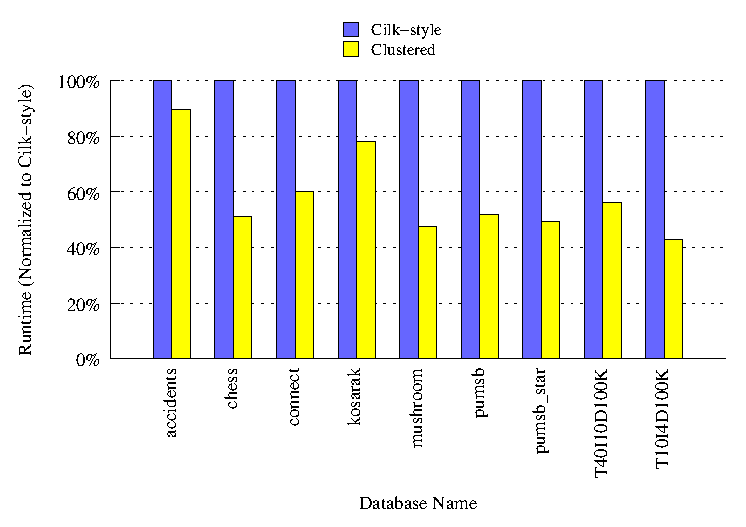
\includegraphics[width=0.5\textwidth]{fimresults/fim_8}
\caption{Graph showing the runtimes (normalized to Cilk-style) of different
datasets when using the Cilk-style and Clustered task scheduling policies in
our Apriori-based frequent pattern mining implementation with 8 threads.
Support for each of the datasets is given in Table~\ref{tbl:fim8}.}
\label{fig:fim8}
\end{figure}

\begin{table*}
\centering
\begin{tabular}{|c|c|c|c|c|c|c|c|}  \hline

\multirow{2}{*}{Dataset} & 
\multirow{2}{*}{Support} & 
\multicolumn{2}{|c|}{Instructions per cycle} &
\multicolumn{2}{|c|}{DTLB L1 miss and L2 hit rate} &
\multicolumn{2}{|c|}{DTLB L1 miss and L2 miss rate} \\ \cline{3-8}
& & Cilk-style & Clustered & 
Cilk-style & Clustered & 
Cilk-style & Clustered \\ 
\hline
accidents & 0.25 &  0.595689 & 0.603959 &
0.000048 & 0.000046 & 0.000161 & 0.000110\\ \hline
chess & 0.6 & 0.560538 & 0.668965 & 
0.000797 & 0.000242 & 0.001006 & 0.000032\\ \hline
connect & 0.8 & 0.543099 & 0.809308 & 
0.000249 & 0.000112 & 0.001204 & 0.000141\\ \hline
kosarak & 0.0013 & 0.692103 & 0.717599 & 
0.000400 & 0.000185 & 0.000659 & 0.000123\\ \hline
pumsb & 0.75 & 0.494539 & 0.719072 & 
0.000230 & 0.000114 & 0.001276 & 0.000126\\ \hline
pumsb\_star & 0.3 & 0.527659 & 0.698358 & 
0.000315 & 0.000145 & 0.001082 & 0.000113\\ \hline
mushroom & 0.10 & 0.570390 & 0.705003 & 
0.000477 &  0.000267 & 0.000950 &0.000022\\ \hline
T40I10D100K & 0.005 & 0.627272 & 0.727288 &
0.000368 & 0.000305 & 0.000900 & 0.000021\\ \hline
T10I4D100K & 0.00006 & 0.555330 & 0.716282 &
0.000218 & 0.000144 & 0.000876 & 0.000044 \\ \hline
\end{tabular}
\caption{Instructions per cycle, L1 data TLB misses and L2 data TLB misses when
using the Cilk-style and Clustered task scheduling policies in our
Apriori-based frequent pattern mining implementation with 8 threads for
different datasets.}
\label{tbl:fim8}
\end{table*}

To experimentally evaluate the benefits of our clustered scheduling policy, we
implemented an Apriori-based frequent pattern application using PFunc and ran
it with both the clustered and the Cilk-style scheduling policies. The
scheduling was selected at compile time using methods described in
Section~\ref{sec:design} and therefore, the frequent pattern mining code itself
required very little modification.  We ran our experiments on a four socket,
quad-core (total 16 cores) AMD 8356 processor running Linux Kernel 2.6.24.  For
compilation, we used GCC 4.3.2 with: ``-O3 -fomit-frame-pointer
-funroll-loops''. To collect hardware metrics, we used PFunc's integration with
PAPI.  The benchmarks were run on data sets from the FIMI
repository~\cite{bart:2004}.

Figure~\ref{fig:fim8} contrasts the runtimes of our Apriori-based frequent
pattern mining implementation for the various data sets with the two scheduling
policies. The results shown are averages after $5$ runs. As can be seen, the
clustered scheduling policy runs significantly faster (more than $50\%$ for
most of the data sets. Only the \code{accidents.dat} data set performs
similarly with both the scheduling policies. To test our hypothesis that our
clustered scheduling policy exploits data locality better than the Cilk-style
policy, we collected various performance measures. Table~\ref{tbl:fim8}
summarizes some of the important metrics. Our clustered scheduling policy
delivers more instructions per clock cycle than the Cilk-style scheduling
policy for all data sets. Also, our clustered scheduling policy incurs far
fewer lower L2 data TLB misses than the Cilk-style scheduling policy. When
results from Figure~\ref{fig:fim8} and Table~\ref{tbl:fim8} are taken together,
we can conclude that the clustered scheduling policy exploits data locality
much better than the Cilk-style scheduling policy for our Apriori-based
frequent pattern mining implementation.

\subsection{Iterative sparse solvers}
\label{sec:cg}
%    - Background and what is the unique requirement placed by this 
%      application
The solution for a sparse system of linear equations, $Ax=b$, is the core
computation in many applications in science and engineering. Krylov-subspace
iterative algorithms, such as CG and GMRES, are an important class of
algorithms to solve such linear systems for sparse matrices.  An efficient
parallel implementation of iterative sparse solvers is best accomplished
through a combination of the SPMD and task-parallel models. Hence,
iterative sparse solvers place unique requirements on parallel programming
tools.  In this case study, we examine those requirements and document the
behavior of an unpreconditioned iterative sparse solver that is parallelized
using different parallel programming models.

\paragraph{Problem description}
Krylov-subspace iterative solvers solve the linear system $Ax=b$ by forming at
each iteration an approximation, $x_i$ of $x$. At iteration $i$ the algorithm
seeks an approximation in the Krylov-subspace $\left\{ b,Ab,\dots
A^{i-1}b\right\} $.  The approximations are formed by manipulating a set of
vectors using two basic operations: matrix-vector multiplication and vector
inner product. Often, a preconditioning phase is added to accelerate the
performance of these iterative solvers. Most preconditioners add another basic
operation to the algorithm: solving sparse triangular systems. 

The SPMD model is especially suited for unpreconditioned iterative sparse
solvers.  First, the vector indices (and, as a consequence, the matrix rows)
are divided among the processors. Each processor is responsible for
manipulating its indices in the vectors. A processor can perform most of the
manipulations and computations independently, but all processors must
synchronize for all the basic operations.  Until all processors reach a certain
point in the computation of those basic operations, no processor can continue.
The amount of data exchanged between processors depends on the number of
non-zeros $A_{ij}$ in $A$ where $i$ and $j$ belong to different processors.
Load balancing depends on the variability in the number of nonzero elements of
the matrix assigned to each processor.  
Graph-partitioning tools like METIS~\cite{MetisPaper} can
efficiently find good data partitionings that enable a well balanced SPMD
implementation with a relatively small amount of data exchange among
processors.
%
For certain types of preconditioners, such as those based on certain incomplete
factorization methods, the triangular solve operations are best parallelized
using the task parallel model (see Section~\ref{sec:dag}).  It is customary to keep the preconditioning
part of the code separate from the solver part so that different
preconditioners and solvers can be mixed and matched to create the desired
combination.

\paragraph{Requirements placed on task parallelism}
We see that Krylov-subspace methods can place a unique requirement on task
parallelism. First, there is an SPMD part, which requires the support of a
barrier.  Then, there is the possibility of calling a task parallel
preconditioning part in each iteration, as a result of which, the program can
alternate between the SPMD and the task parallel parts.  Therefore, it is
important to have the right synchronization constructs that support these
functionalities.

\paragraph{Shortcomings of existing models}
Existing implementations of task parallelism perceive tasks as independent
entities that typically do not interact with each other directly.  Often, this
forces users to construct higher-level task synchronization constructs from the
native locks.  For example, Cilk provides a spin lock that may be used by
skilled parallel programmers to construct a barrier, but it does not provide
direct support for synchronization.  To implement the SPMD version of an
iterative sparse solver without locks, the barrier synchronization has to be effected
by decreasing the granularity of the tasks; that is, new tasks must be created
and destroyed between each synchronization point in each iteration.

Current solutions for task parallelism favor parallelizing the basic
operations using a divide-and-conquer approach.  Such an implementation is
more complex, especially for sparse matrix-vector multiplication
operation, and incurs more synchronization points than the SPMD version.
Without the benefit of graph-partitioning induced
locality, it may also suffer from poor cache utilization.

%    - Description of how this can be done using PFunc's new features.
\paragraph{PFunc's approach}
PFunc's support for task groups (Section~\ref{sec:groups}) allows natural
parallelization of both the preconditioned and the unpreconditioned algorithms.
First, a task group of $n$ tasks are created where $n$ is the number of CPUs.
Each task works on different indices governed by its rank in the task group.
Upon encountering a synchronization point, the tasks synchronize via the
barrier construct provided by PFunc.  In case a task-parallel preconditioner
with a triangular solve is required, a single task with a predefined rank calls the solve
function followed by a spinning barrier.  The tasks with all other ranks call a
stealing barrier (Section~\ref{sec:groups}), which enables the threads
executing these tasks to temporarily relinquish them and execute the tasks
spawned from the task-parallel solve function.  All tasks return to the barrier
upon the completion of the solve.

\paragraph{Experimental results}
To study the effect of the model of parallelism used in parallelizing the CG
iterative sparse solver (unpreconditioned), we implemented three different
parallel solutions. The first solution was purely SPMD and was implemented with
the aid of OpenMP's \code{parallel} and \code{barrier} constructs. The second
solution was that of PFunc's task groups, which synchronized with each other
using the task-level barrier construct.  The third solution was a purely
task-based SPMD-spirited solution implemented in Cilk.  The tests were run on a
four socket, quad-core AMD 8356 processor running Linux Kernel 2.6.24.  For the
OpenMP and PFunc versions, we used the GCC 4.3.2 compiler. For the Cilk model,
we used Cilk 5.4.6. The following compilation flags were used: "-O3
-fomit-frame-pointer -funroll-loops -fschedule-insns2".  For benchmarking, we
used matrices from the University of Florida collection~\cite{davissparse}.

\begin{figure}[t]
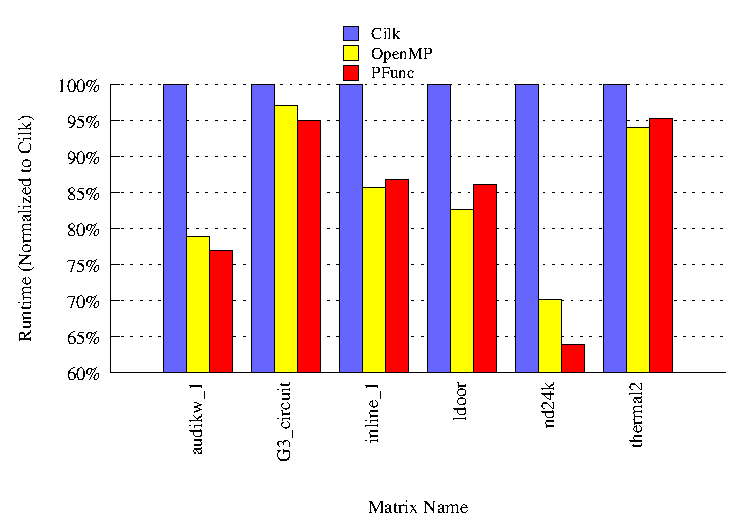
\includegraphics[width=0.5\textwidth]{cgresults/cg_8}
\caption{Execution times (normalized to Cilk) of Cilk, OpenMP and PFunc
implementations of CG for different sparse matrices with 8 threads.}
\label{fig:cg8}
\end{figure}

Figure~\ref{fig:cg8} shows the runtimes of the three implementations of the
unpreconditioned CG method normalized to the Cilk runtime with 8 threads. 
For the sake of perusal of the variations in the runtimes of the three
implementations, the y-axis in Figure~\ref{fig:cg8} has been started at $60\%$.
For most of the benchmark matrices, the OpenMP and the PFunc implementations
perform better than the Cilk implementation by at least $10\%$. In fact, for
the \code{audi\_kw1} and \code{ldoor} matrices, the performance difference is
significantly higher ($28\%$ and $50\%$ respectively). Our experiments lead to
two conclusions: first, that the model of task parallelism chosen for
parallelization has an impact on the performance of the iterative sparse
solvers and second, the SPMD model of parallelism can be elegantly incorporated
into the task parallel model with no performance penalties.

\section{Conclusions}
\label{sec:conclusion}
We present PFunc, a new parallel library for task parallelism that
increases the support for modern HPC applications over current solutions for
task parallelism.  By means of three case studies, we show that PFunc
performs better than current solutions.  We see that PFunc is able to
smoothly incorporate support for existing SPMD algorithms within its task
parallel model. This equips users with a great deal of flexibility in
implementing their algorithms.  PFunc is able to achieve these milestones by
introducing new features such as custom task scheduling, task priorities, task
affinities, multiple completion notifications and task groups. By using
generative and generic programming principles, PFunc offers customizations to
the users without incurring any runtime penalties.

We are currently evaluting several interesting opportunities that exist to
enhance PFunc and broaden its scope.  We can easily extend the support for the
SPMD model by introducing features to enhance cooperation and communication
among tasks.  PFunc can be naturally extended to support GPGPUs by means of
special queue types implemented using OpenCL~\cite{MUNSHI08siggraph}. This will
provide users a productive environment for developing high-performance programs
that are portable between GPGPUs and regular multi-core CPUs.  PFunc's
interface has been carefully designed so as to behave uniformly across shared-
and distributed-memory architectures.  An important area for future work is to
implement a distributed-memory version of PFunc.

\section{Acknowledgments}
We thank Joseph Cottam, Jeremiah Willcock, Torsten Hoefler and Nicholas Edmonds
for valuable insights that improved the quality of this paper.  This work was
supported by IBM, King Abdullah University of Science and Technology (KAUST),
National Science Foundation grants EIA-0202048 and CCF-0541335, and a grant
from the Lilly Endowment.

\small
\bibliographystyle{plain}
\bibliography{refs}

\end{document}
